\subsection{Chi-Square Distance}

The chi-square distance is often used in textual data analysis to find similarities between documents. It is very close to the euclidean distance (sum of squared differences between the elements) weighted by a term associated to the frequency of each word in the whole corpus.

\subsubsection{The formula}

In each subset $C_i$ of the corpus, we can denote $f_{i,j}$ the frequency of the word $w_j$. The distance is computed as follows:
\begin{eqnarray}
 d(C_i,C_{i'}) = \sum_j \frac{1}{f_{.j}} (\frac{f_{i,j}}{f_{i.}} - \frac{f_{i',j}}{f_{i'.}})^2
\end{eqnarray}
where $f_{i.} = \sum_j f_{i,j}$ is the total number of words contained in $C_i$ and $f_{.j} = \sum_i f_{i,j}$ is the frequency of the word $w_j$ over the entire corpus.

The term $f_{i,j}$ can also be replaced by the TF-IDF term.

\subsubsection{Computations on the corpus}

We applied the chi-square distance on the years contained in the corrected corpus, producing the following matrix:

\begin{figure}[H]
    \begin{minipage}[b]{0.48\linewidth}
        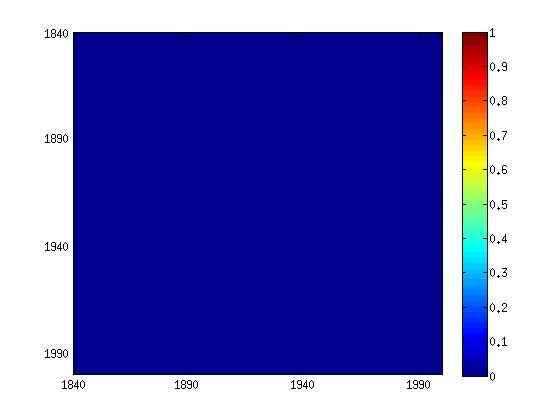
\includegraphics[scale=0.3]{Pictures/chi2/chi2_corrected2.jpg}
        \caption{chi-square distance for 1-gram with OCR correction}
        \label{chi2_1}
    \end{minipage}\hfill
    \begin{minipage}[b]{0.5\linewidth}
        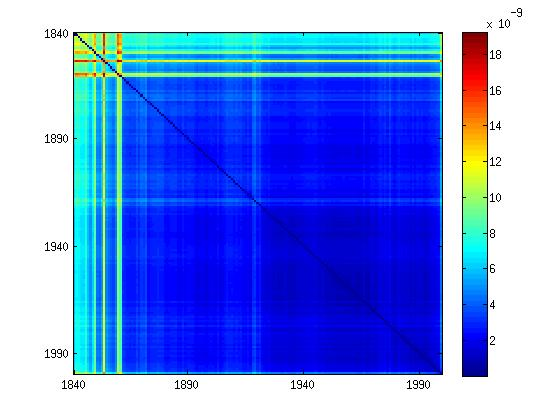
\includegraphics[scale=0.3]{Pictures/chi2/chi2_corrected.jpg}
        \caption{chi-square distance with reduced scale}
        \label{chi2_2}
    \end{minipage}\hfill
\end{figure}
\begin{figure}[H]
    \begin{minipage}[b]{0.48\linewidth}
        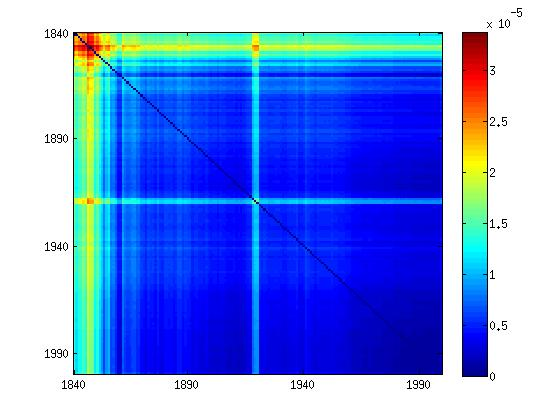
\includegraphics[scale=0.3]{Pictures/chi2/chi2_corrected_tfidf.jpg}
        \caption{chi-square distance weighted by TF-IDF}
        \label{chi2_tfidf}
    \end{minipage}\hfill
\end{figure}

\subsubsection{Analysis}

As we have a huge amount of articles for each year and that chi-square is used to compare documents, the maximal distance achieved is very low as shown in figure \ref{chi2_1}. In order to observe something we reduced the scale of the colours in figure \ref{chi2_2}. This distance is definitively smoother than the basic one but it doesn't show any evolution through the years.

Figure \ref{chi2_tfidf} shows the results when the terms of the distance are weighted by the TF-IDF coefficients. The values look similar than without the weighting.